% !Mode:: "TeX:UTF-8"

\chapter{}
\textbf{
Suppose you're consulting for a company that manufactures PC equipment and ships it to distributors all over the country. For each of the next $n$ weeks, they have a projected \emph{supply} $s_i$ of equipment(measured in pounds), which has to be shipped by an air freight carrier.
}

\textbf{
Each week's supply can be carried by one of two air freight companies, A or B.
}

\textbf{
\begin{itemize}
  \item Company A charges a fixed rate $r$ per pound(so it costs $r\cdot s_i$ to ship a week's supply $s_i$).
  \item Company B makes contracts for a fixed amount $c$ per week, independent of the weight. However, contracts with company B must be made in blocks of four consecutive weeks at a time.
\end{itemize}
}

\textbf{
A \emph{schedule}, for the PC company, is a choice of air freight company (A or B) for each of the $n$ weeks, with the restriction that company B, whenever it is chosen, must be chosen for blocks of four contiguous weeks at a time. The \emph{cost} of the schedule is the total amount paid to company A and B, according to the description above.
}

\textbf{
Give a polynomial-time algorithm that takes a sequence of supply values $s_1,s_2,...,s_n$ and returns a \emph{schedule} of minimum cost.
}

\noindent
\textbf{
Example. Suppose $r=1$, $c=10$, and the sequence of values is
}

\textbf{
$$11,9,9,12,12,12,12,9,9,11.$$
}

\noindent
\textbf{
Then the optimal schedule would be to choose company A f or the first three weeks, then company B for a block of four consecutive weeks, and then company A for the final three weeks.
}

\hspace*{\fill} \\
Let $M_i$ be the total cost when there a sequence of $i$ supply values $s_1,...,s_i$. Then we have

\begin{equation}
M_i=
\left\{
             \begin{array}{lr}
             0,
             & i=0 \\
             min\{4c,M_{i-1}+rs_i\},
             & 1\leq i\leq 3\\
             min\{M_{i-4}+4c,M_{i-1}+rs_i\},
             & i\geq 4
             \end{array}
\right.
\end{equation}

We design a list to record each step and the precursor message. The algorithm is showed in~\ref{alg_1}.

\begin{algorithm}
\caption{Optimal schedule}
\label{alg_1}
\begin{algorithmic}[1]
\REQUIRE a series supplies $s_1,...,s_n$
\STATE Initialize array $data$ to be a empty list
\FOR{$i=1$ to $n$}
    \IF{$i == 0$}
        \STATE{Set $data[i]$ to $(0,0)$}
    \ELSIF{$1\leq i \leq 4$}
        \IF{$4c<M_{i-1}+s_i$}
            \STATE{Set $a$ to -4}
            \STATE{Set $data[i]$ to $(a,4c)$}
        \ELSE
            \STATE{Set $a$ to -1}
            \STATE{Set $data[i]$ to $(a,M_{i-1}+s_i)$}
        \ENDIF
    \ELSE
        \IF{$M_{i-4}+4c<M_{i-1}+s_i$}
            \STATE{Set $a$ to -4}
            \STATE{Set $data[i]$ to $(a,M_{i-4}+4c)$}
        \ELSE
            \STATE{Set $a$ to -1}
            \STATE{Set $data[i]$ to $(a,M_{i-1}+s_i)$}
        \ENDIF
    \ENDIF
\ENDFOR
\STATE{Initialize an array $W$}
\STATE{Initialize $k$ as $data[n][1]$}
\STATE{Initialize $m$ as $n$}
\STATE{Initialize $i$ as $0$}
\WHILE{$m>0$}
    \IF{$k == -3$}
        \STATE{$W[i]=B$}
        \STATE{$m = m - 4$}
    \ELSE
        \STATE{$W[i]=A$}
        \STATE{$m = m - 1$}
    \ENDIF
    \STATE{$i = i + 1$}
\ENDWHILE
\STATE{Reverse $W$}
\STATE{Return $data[n][2]$ and $W$}

\end{algorithmic}
\end{algorithm}

It is to see that the process of getting minimum value and backtracking route are both $O(n)$.

%\begin{figure}[!htbp]
%\centering
%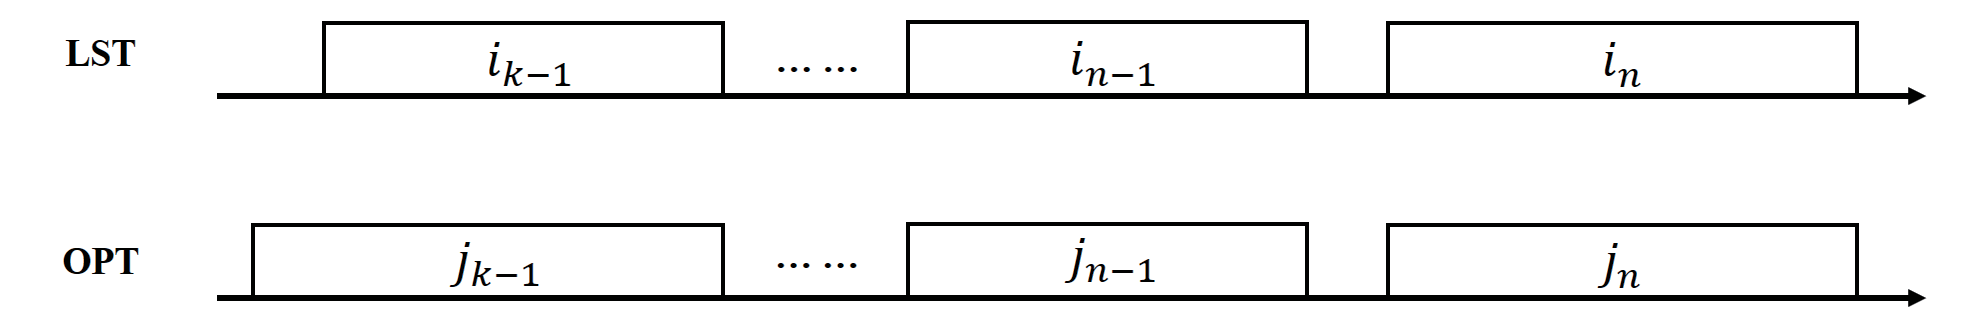
\includegraphics[width=1\textwidth]{figures/1.eps}
%\caption{A way of Optimal choice Vs the way of last activity to start}\label{fig_1_1}
%\end{figure}
